%\PassOptionsToPackage{demo}{graphicx}
\documentclass[slidestop,compress,11pt,xcolor=dvipsnames]{beamer}
%\documentclass{beamer}
\usepackage[latin1]{inputenc} % remplace utf8 con latin1 si va a compilar en un sistema Windows
\usepackage{times}
\usepackage{mdframed}
\usepackage[T1]{fontenc}
\usepackage[spanish]{babel}
\usepackage[sort]{natbib}
\usepackage{textpos}
%\usepackage{graphicx} %sirve para insertar graficos en varios formatos%
\usepackage{graphicx}
%\usepackage{subcaption}
\usepackage{mathtools}
\usepackage[bars]{beamerthemetree} % Beamer theme v 2.2
\usepackage{multicol}
\usepackage{lmodern}
\usepackage{lipsum}
\usepackage{marvosym}
\usefonttheme{professionalfonts} % font de Latex
%\DeclareGraphicsRule{.png}{png}{.png.bb}{} %al parecer sirve para adaptar el tama�o de los gr�ficos cuando se insertan en Beamer
%\usepackage{beamerthemeshadow} %hay que descargar est� opci�n
\newtheorem{defi}{Definici�n}
\setbeamertemplate{navigation symbols}{}
\setbeamertemplate{caption}[numbered]
\providecommand{\abs}[1]{\lvert#1\rvert}
\providecommand{\norm}[1]{\lVert#1\rVert}

% Agregamos informaci�n del autor y titulo

\title[Intro. Econom�a]
{Introducci�n a la Econom�a - semestre I de 2015 \\
Clase \#3 - El economista como cient�fico y su papel en la econom�a}

\author[Prof. Andr�s M. Casta�o]
{
\includegraphics[height=2cm,width=2.5cm]{ucn.jpg}
\\
% con el del mcr es height=1.5cm,width=4cm
Andr�s M. Casta�o}

\institute[]
{
}

\LARGE
\date[Clase 3 ]
{INGECO \\
 INGESIS \\
Universidad Cat�lica del Norte\\
}

%\date{\today}

%Definimos la apariencia de las presentaciones
%para agregar la l�nea de informaci�n en la diapositiva
\setbeamercolor{block title}{bg=red!60,fg=black}
\useoutertheme{infolines}
\usetheme{Boadilla} %tipo de tema
%\usecolortheme{whale} %color del tema
\usecolortheme{orchid}
\setbeamercovered{dynamic} % dentro de ambientes como itemize o enumerate resalta uno y los demas los pone trasparantes
\useoutertheme{infolines}
\useinnertheme{default} % aspectos dentro del tema (cajas, vi�etas, itemize, enumerate, theorem, footnotes. bibliography. opciones: circles,
% default, rectangles


\begin{document} %inicio del documento


%portada
\begin{frame}
\titlepage
\end{frame}

%indice
%\begin{frame}
%\frametitle{Contenido}
%\tableofcontents[pausesections]
%\end{frame}

%\AtBeginSubsection[]
%{
%\begin{frame}{Contenido}
%\tableofcontents[currentsection,currentsubsection,currentsubsubsection]
%\end{frame}
%}

%\addtobeamertemplate{footline}{\hfill\insertframenumber/\inserttotalframenumber\hspace{2em}\null}
%\addtobeamertemplate{footline}{\insertframenumber/\inserttotalframenumber}
%\inserttotalframenumber

\section{El economista como cient�fico}
\begin{frame}
\frametitle{El economista como cientifico}
\begin{itemize}
\item <1> Qu� significa pensar como un economista?.\\
\bigskip
\item <2> La esencia de la ciencia es el m�todo cient�fico.\\
\bigskip
\item <3> Ciencias sociales vs. ciencias naturales.
\bigskip
\item <4> La importancia de los experimentos naturales
\bigskip
\item <5> Construcci�n de modelos $\Longrightarrow$ El rol de los supuestos y su validez
\begin{itemize}
\bigskip
\item <5> Planteamiento directo $\Longrightarrow$ validez de los supuestos
\item <5> Planteamiento indirecto $\Longrightarrow$ Que pueda predecir la realidad
\end{itemize}
\end{itemize}
\end{frame}

\begin{frame}
\frametitle{\textbf{Nuestro primer modelo:} el diagrama de flujo circular}
\begin{center}
\begin{figure}
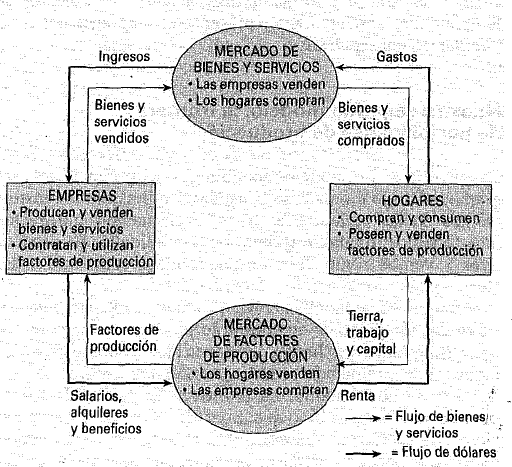
\includegraphics[width=8cm]{diagrama}
\end{figure}
\end{center}
\end{frame}

\begin{frame}
	\frametitle{\textbf{Nuestro segundo modelo:} la frontera de posibilidades de producci�n (lineal)}
	\begin{center}
		\begin{figure}
			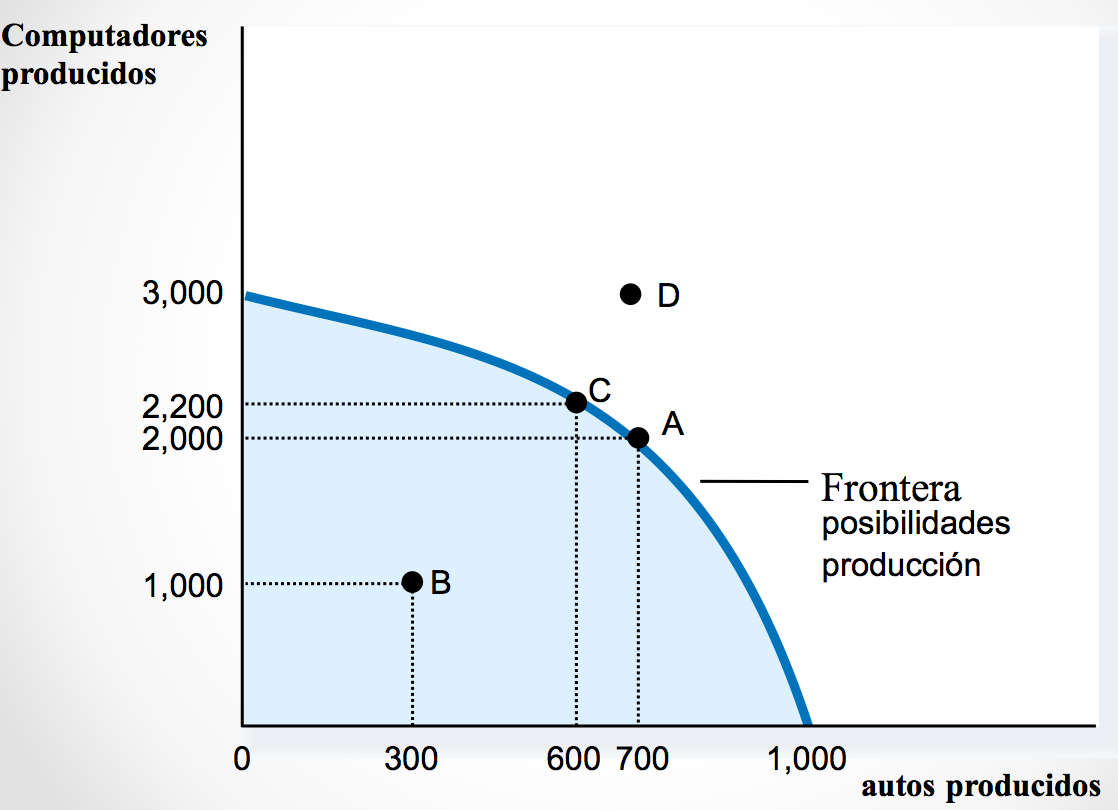
\includegraphics[width=10cm]{frontera3}
		\end{figure}
	\end{center}
\end{frame}

\begin{frame}
\frametitle{\textbf{Nuestro segundo modelo:} la frontera de posibilidades de producci�n}
\begin{center}
\begin{figure}
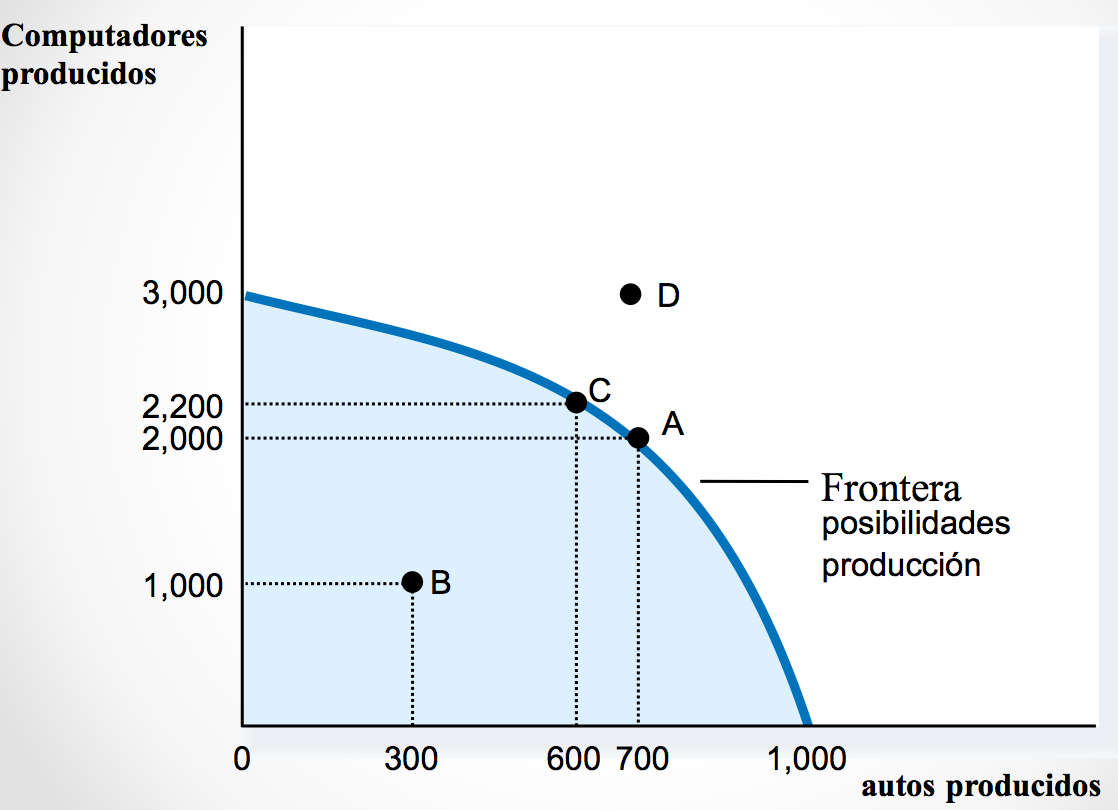
\includegraphics[width=10cm]{frontera3}
\end{figure}
\end{center}
\end{frame}

\begin{frame}
\frametitle{\textbf{Nuestro segundo modelo:} la frontera de posibilidades de producci�n}
\begin{center}
\begin{figure}
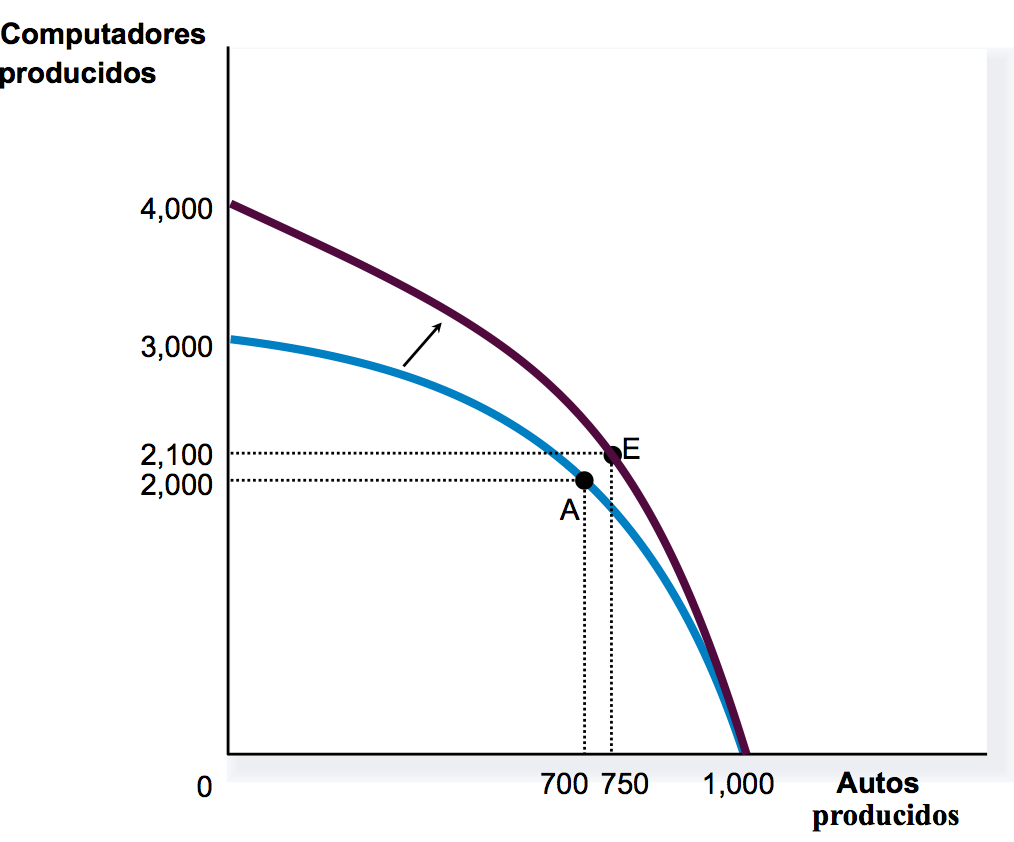
\includegraphics[width=9cm]{frontera4}
\end{figure}
\end{center}
\end{frame}

\begin{frame}
\frametitle{Niveles de estudio de la econom�a}
\centering
\begin{itemize}
\item <1> \textbf{Microeconom�a:} Es el estudio de la econom�a al nivel de los consumidores individuales, grupos de consumidores, o empresas, con el fin de determinar la asignaci�n eficiente de recursos escasos entre usos alternativos.
\bigskip
\item <2> Piense ahora: �Qu� ser�a la macroeconom�a?
\end{itemize}
\end{frame}

\begin{frame}
\frametitle{Se entendi� la diferencia?}
\begin{center}
\begin{figure}
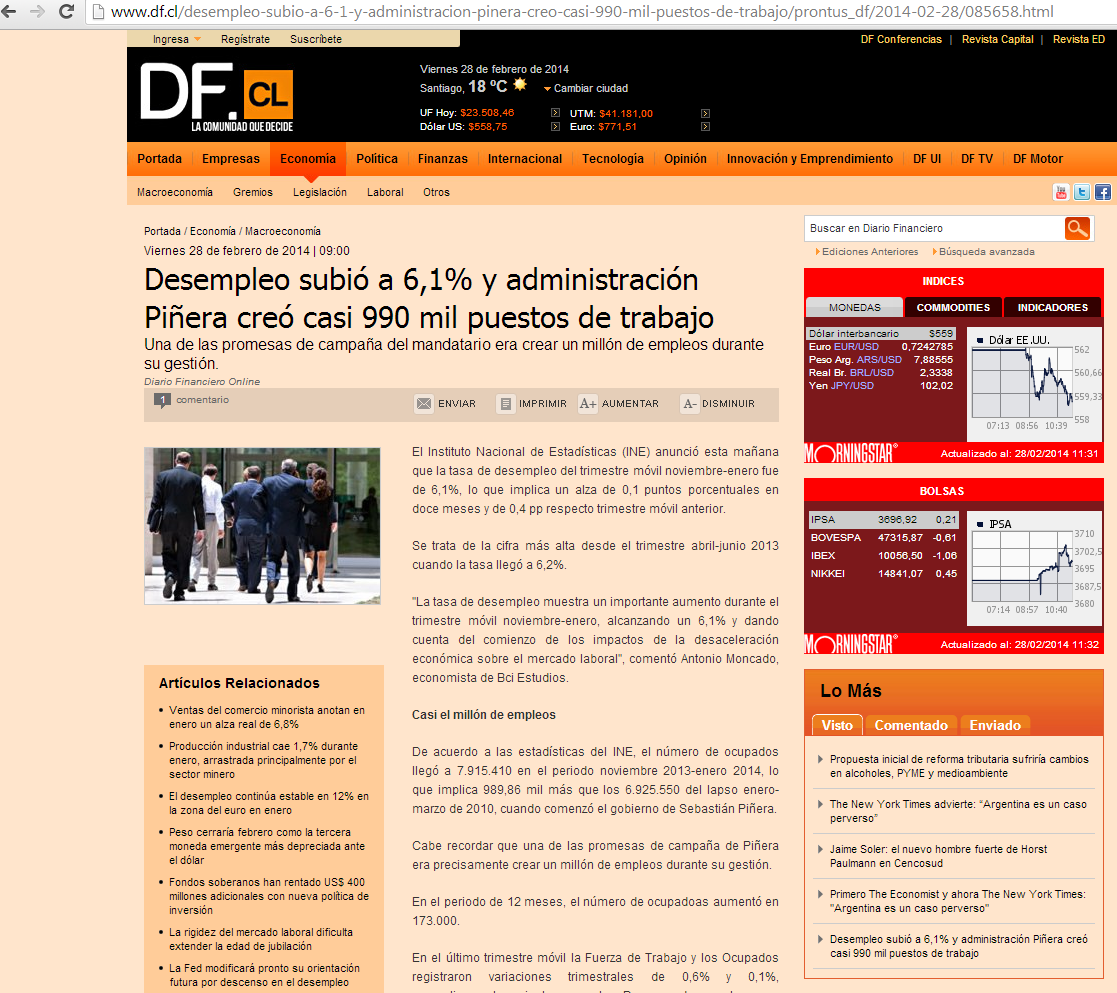
\includegraphics[width=10cm]{Macro1}
\end{figure}
\end{center}
\end{frame}

\begin{frame}
\frametitle{Micro o macro?}
\begin{center}
\begin{figure}
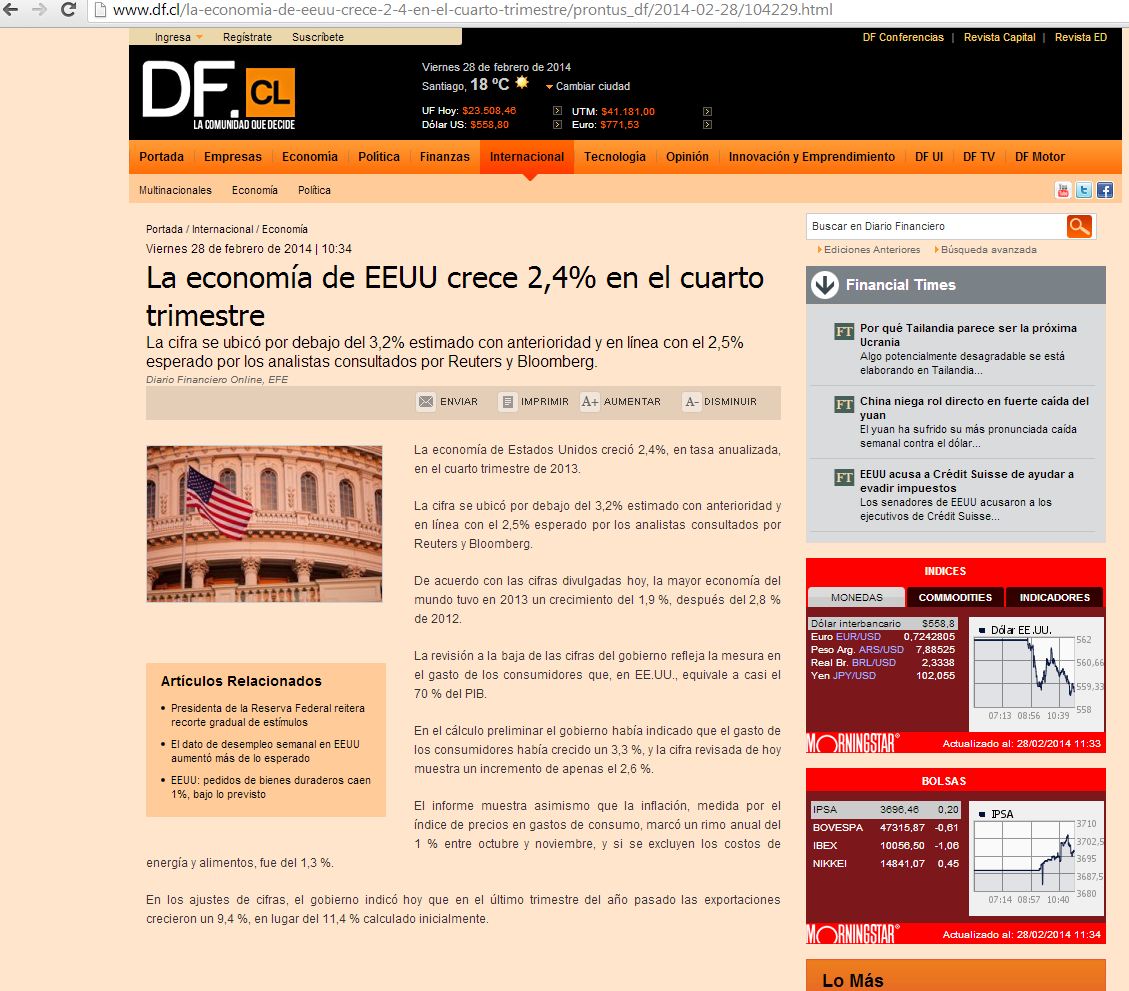
\includegraphics[width=10cm]{Macro2}
\end{figure}
\end{center}
\end{frame}

\begin{frame}
\frametitle{Micro o macro?}
\begin{center}
\begin{figure}
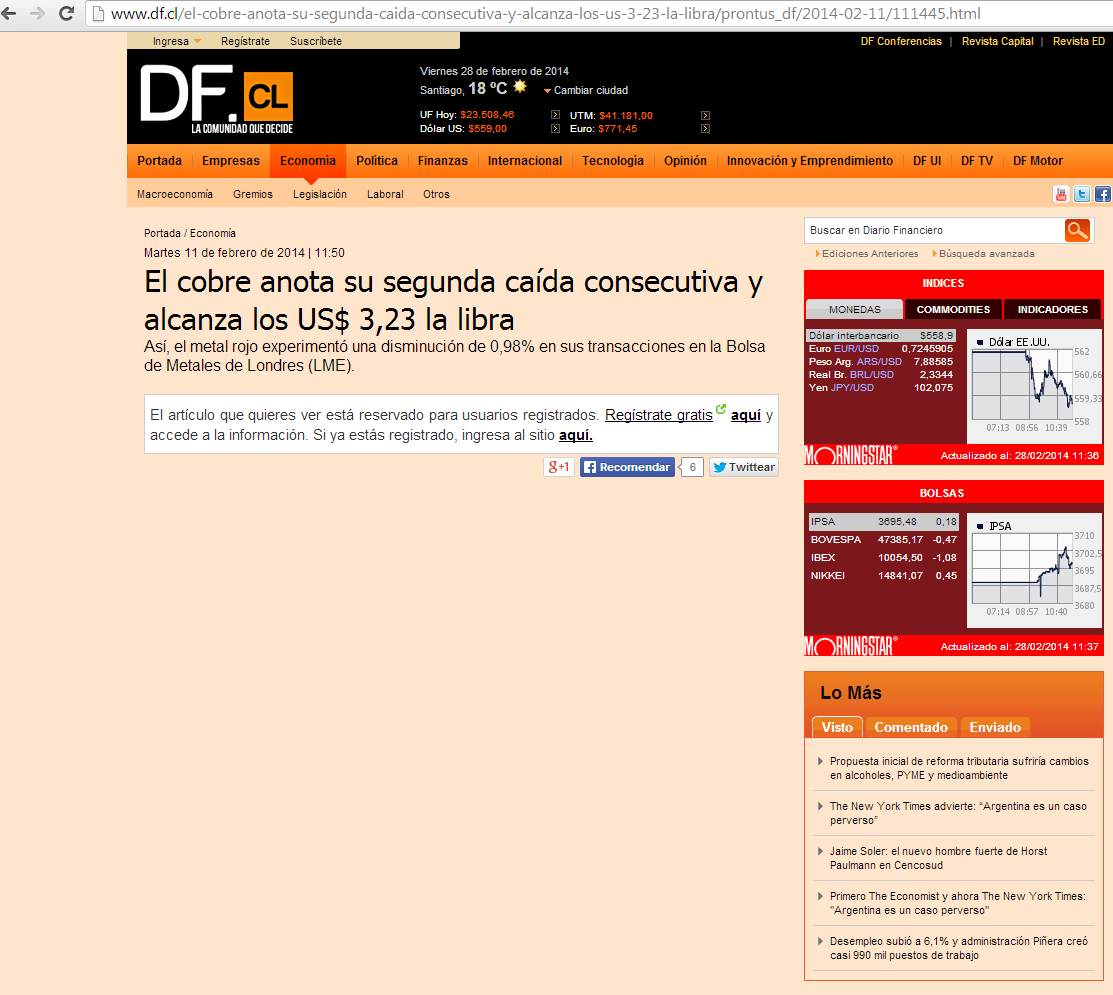
\includegraphics[width=10cm]{Micro1}
\end{figure}
\end{center}
\end{frame}

\begin{frame}
\frametitle{Micro o macro?}
\begin{center}
\begin{figure}
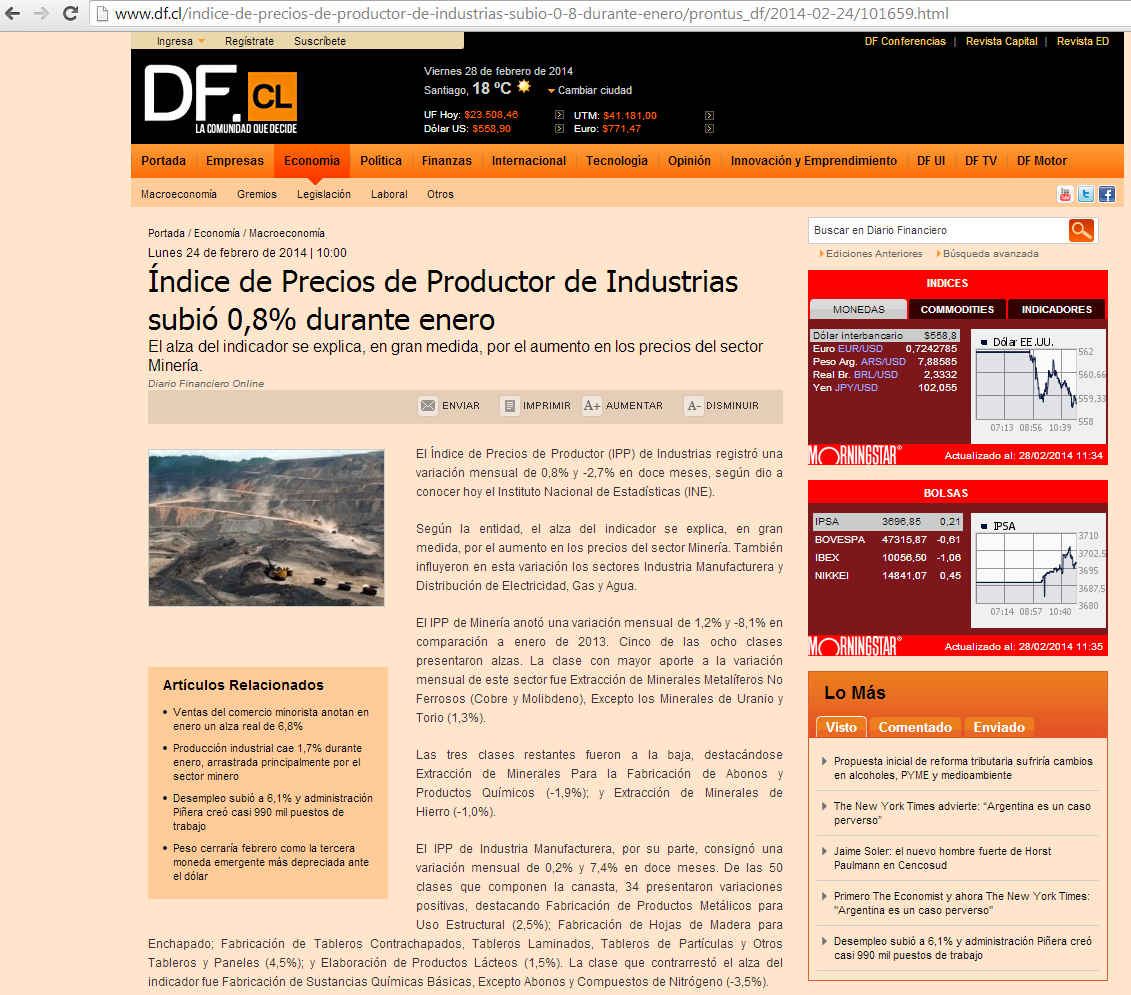
\includegraphics[width=10cm]{Macro3}
\end{figure}
\end{center}
\end{frame}

\begin{frame}
\frametitle{Micro o macro?}
\begin{center}
\begin{figure}
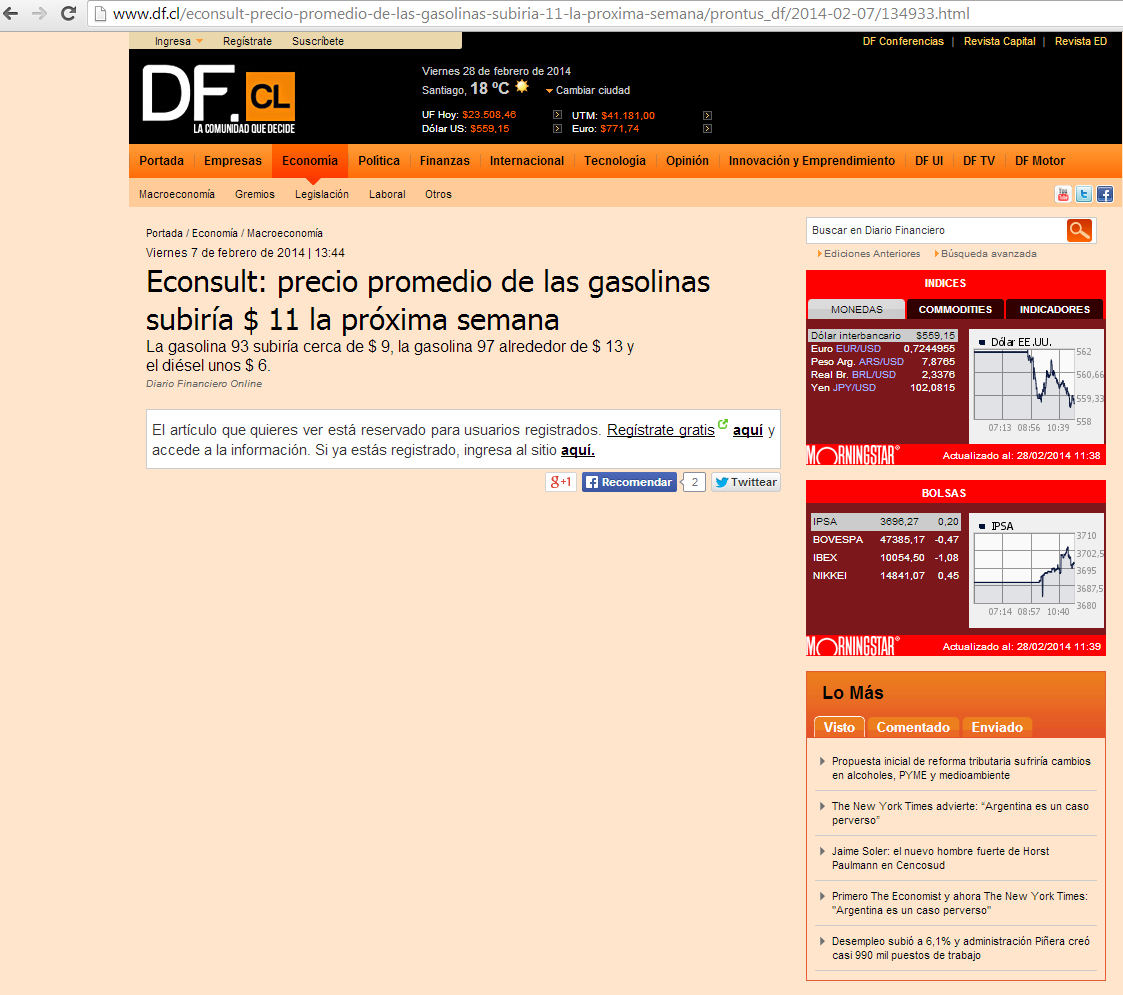
\includegraphics[width=10cm]{Micro2}
\end{figure}
\end{center}
\end{frame}

\begin{frame}
\frametitle{Micro o macro?}
\begin{center}
\begin{figure}
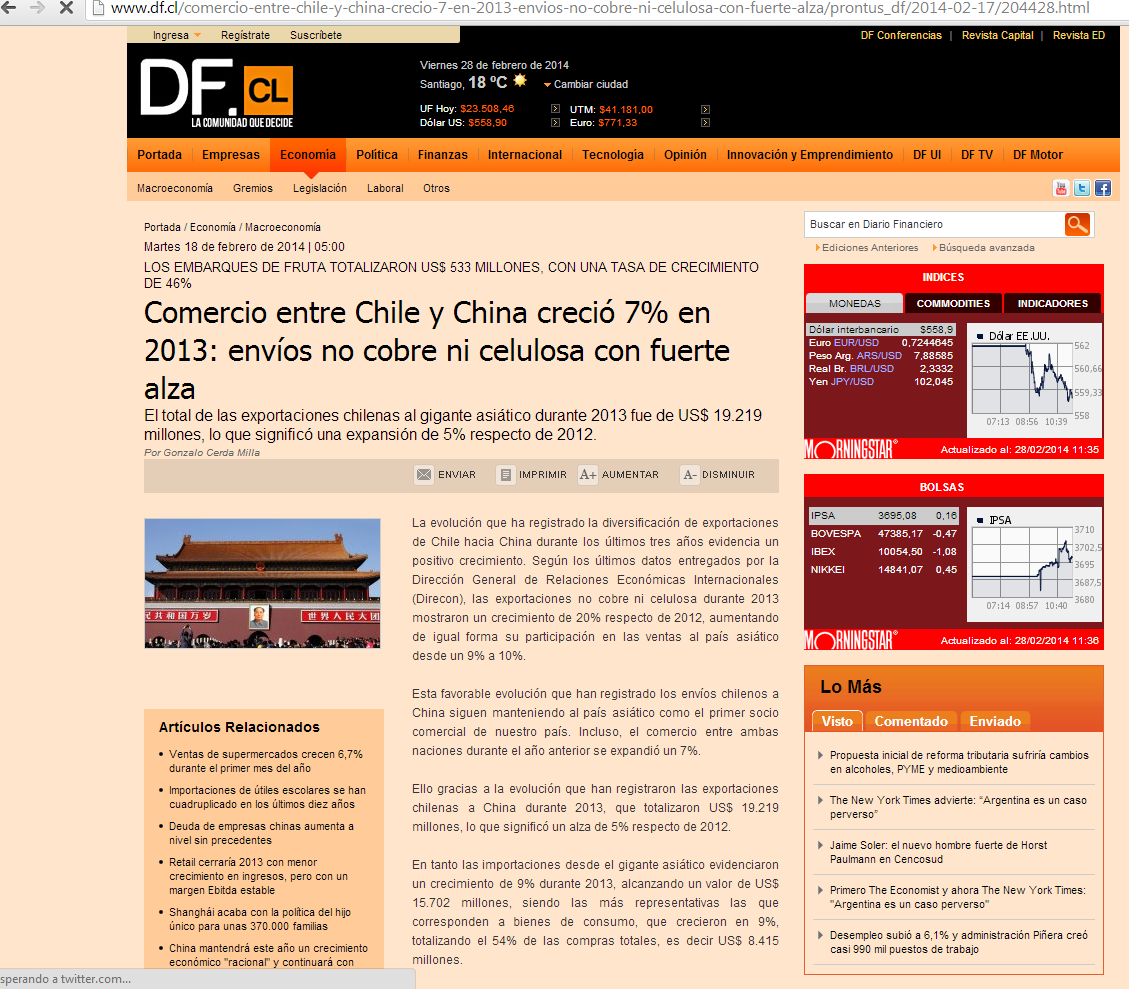
\includegraphics[width=10cm]{Macro4}
\end{figure}
\end{center}
\end{frame}


\end{document} %fin del documento
